\documentclass[12pt,a4paper]{report}
\usepackage[latin1]{inputenc}
\usepackage[spanish,es-tabla]{babel}
\usepackage{graphicx}
\usepackage[left=3cm,right=3cm,top=2.5cm,bottom=2.5cm]{geometry}
\usepackage{lastpage}
\usepackage{fancyhdr}
\pagestyle{fancy}
\fancyhead[R]{\textbf{\thepage/\pageref{LastPage}}}
\renewcommand{\headrulewidth}{0pt}

\begin{document}
\begin{titlepage}
\begin{center}
\vspace*{1.5cm}
\textbf{Escuela de Ingeniería en Electrónica}\\[0.8cm]
\textbf{Laboratorio de Diseño de Sistemas Digitales}\\[1cm]
\textbf{Bitácora}\\[2cm]
\textbf{Proyecto:}\\[0.4cm]
Control y programación RTC con Nexys3 \\[1.7cm]
\textbf{Profesor:}\\[0.4cm]
Alfonso Chacón Rodríguez \\[1.7cm]
\textbf{Estudiantes:}\\[0.4cm]
Keylor Mena Venegas \\[0.8cm]
Luis Leon Vega \\[0.8cm]
Luis Merayo Gatica \\[1.7cm]
\textbf{Periodo}\\[0.8cm]
II Semestre, 2016\\
\end{center}
\end{titlepage}


\section*{\textit{Descripción del problema}}

Se debe realizar un controlador para realizar la lectura y escritura del módulo RTC V3023. Los datos del sistema deben poder ser desplegados en un monitor LCD mediante el protocolo VGA. Ante ello, se debe realizar un controlador para el RTC y para la VGA. Asimismo, se deben poder ajustar la hora, activar la alarma y el cronómetro de forma descendente mediante botones e interruptores dispuestos en la FPGA Nexys3.

\section*{\textit{Introducción al proyecto}}

Este proyecto consiste en realizar un controlador de módulos RTC (Real Time Controller), específicamente para el módulo V3023. Este controlador será capaz de escribir y leer dicho módulo para obtener parámetros de reloj, cronómetro y alarma. \\
Asimismo, para poder desplegar la información relevante de los parámetros anteriores, se conectará un monitor LCD mediante el protocolo VGA. Por otro lado, para poder programar y dar instrucciones al circuito, se deberán usar los botones señalados en el instructivo y algunos interruptores. \\
Finalmente, el conjunto es un circuito que permita controlar el módulo y comunicar al usuario mediante los botones y el monitor LCD, donde él podrá recibir la información relevante y poder modificar dicha información.\\

\section*{\textit{Objetivo General}}
Diseñar un controlador de RTC que permita leerlo y programarlo mediante una interfaz de usuario consistente en botones incorporados dentro de la FPGA (Nexys3) y un monitor comunicado a través del protocolo VGA.

\section*{\textit{Objetivos Específicos}}
\begin{itemize}
\item Investigar el funcionamiento del módulo RTC y el protocolo de comunicación del mismo.
\item Diseñar un controlador para el módulo RTC, cuyo bus de datos y direcciones estén multiplexados.
\item Cumplir con las reglas de temporizado del sistema, en especial, con el protocolo de comunicación del módulo RTC.
\item Combinar el controlador de RTC con un controlador VGA para poder desplegar la información del módulo al usuario. Este módulo VGA será adaptado del proyecto anterior.
\item Desarrollar un banco de pruebas (testbench) para poder emular el comportamiento del módulo RTC con la finalidad de comprobar el funcionamiento del circuito controlador.
\end{itemize}

\newpage

% Comienzo de la bitacora
\section*{\textit{Control de eventos}}

% Nueva entrada
\begin{flushright}
	\begin{large}
		\textbf{Fecha: 30 de Agosto}\\[5ex]
	\end{large}
\end{flushright}

\noindent \textbf{Integrantes:} Luis Leon, Luis Merayo, Keylor Mena \\[1ex]
\textbf{Hora:} 13:00 - 15:00 \\[1ex]
\textbf{Actividad:} \\[2ex]

El profesor explicó el instructivo y expresó las necesidades que deben ser cubiertas durante todo el proyecto. Quedó claro en que se debe desarrollar unidades de control para el proyecto (que se pueden hacer con FSM o Máquinas de Estados Finita) y desarrollar un controlador para obtener datos del RTC y para programarlo. \\

t El reto de este último surge, principalmente, de comunicar el circuito al RTC mediante un bus multiplexado de direcciones y datos (A/D Bus). Se debe crear un control que permita escribir y leer de forma controlada y, con ello, que se pueda seleccionar el hardware para cada caso. \\

\indent En este día, se hizo una reunión grupal para decidir las tareas de cada miembro, lo cual estableció: 

\begin{itemize}
	\item Luis Leon: Control general del circuito - Controlador VGA
	\item Luis Merayo: Control del RTC
	\item Keylor Mena: Encargado de testbench.
\end{itemize}

No se estableció ninguna aproximación al diseño del proyecto para dar tiempo de que cada miembro pueda estudiar el instructivo y el RTC con calma y de forma individual. Asimismo, se quedó que el día de mañana, esta tarea será efectuada al igual que la distribución de todas las tareas que puede implicar el proyecto. \\

Sin embargo, se ha decido usar el control VGA que se ha diseñado en el proyecto anterior para agilizar la tarea del nuevo diseño de proyecto, asumiendo de que se conocen todas las partes de este controlador. Por otro lado, para efectos de la comprensión del nuevo proyecto, se asistió a la tutoría el día anterior, brindando la facilidad de que uno de los miembros conozca el sistema de antemano. Para ello será recomendado ver el enlace de interés al final de esta entrada. \\

\noindent \textbf{Enlaces de interés:}
\begin{itemize}
	
	\item Documento de la tutoría: http://bit.ly/2bEI3RZ
	\item Datasheet del RTC: http://bit.ly/2cpNGJa
\end{itemize}

\newpage

% Nueva entrada
\begin{flushright}
	\begin{large}
		\textbf{Fecha: 31 de Agosto}\\[5ex]
	\end{large}
\end{flushright}

\noindent \textbf{Integrantes:} Luis Leon \\[1ex]
\textbf{Hora:} 7:30 - 8:00 \\[1ex]
\textbf{Actividad:} \\[2ex]

Se incorporaron los apartados de descripción del problema, introducción al proyecto y los objetivos dentro del documento de control de eventos (bitácora). Esto para seguir el formato de la plantilla proporcionada por el profesor. \\[2ex]

% Nueva entrada
\begin{flushright}
	\begin{large}
		\textbf{Fecha: 1 de Septiembre}\\[5ex]
	\end{large}
\end{flushright}

\noindent \textbf{Integrantes:} Keylor Mena, Luis Leon, Luis Merayo \\[1ex]
\textbf{Hora:} 8:00-9:00\\[1ex]
\textbf{Actividad:} \\[2ex]

Se realizó una reunión de todos los miembros del grupo, donde se plasmaron las ideas del control del RTC y se establecieron las comunicaciones entre los módulos principales, donde se destacan \\

\begin{enumerate}
	\item Control VGA
	\item Control de Usuario
	\item Control de Memoria
	\item Control de RTC
\end{enumerate}

Como parte del protocolo, se estableció una comunicación entre el control principal (de Memoria) con el control RTC, ilustrado en la siguiente imagen de la Figura \ref{fig:protocolRTC} \\

\begin{figure}[hbtp]
	\centering
	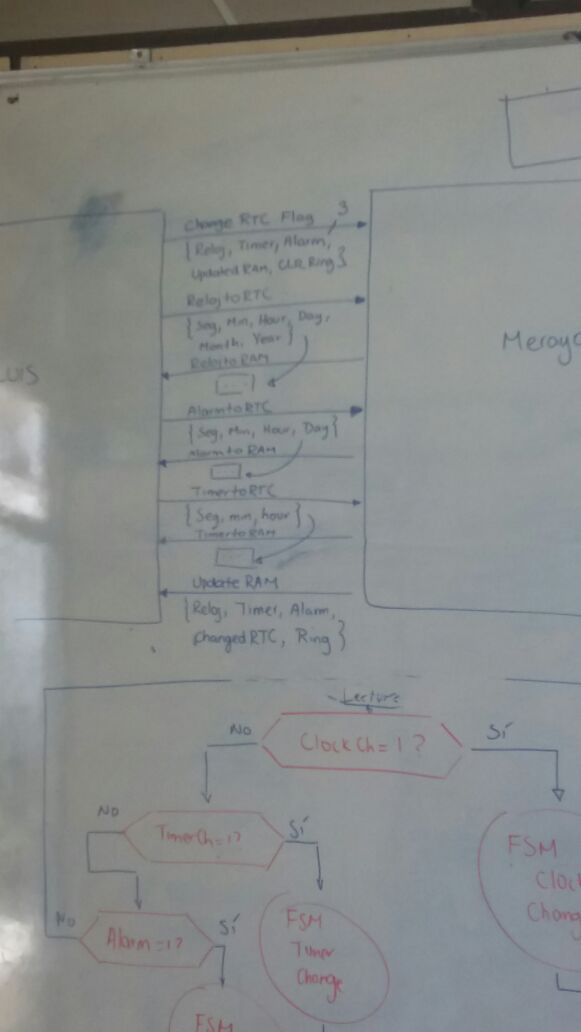
\includegraphics[width=14cm]{Img/protocolRTC.jpeg}
	\caption{Diagrama de protocolo}
	\label{fig:protocolRTC}
\end{figure}

Por otro lado, se hizo un acercamiento al diagrama de flujo del módulo de RTC, mostrado en la Figura \ref{fig:RTCdiagramaflujo} \\

\begin{figure}[hbtp]
	\centering
	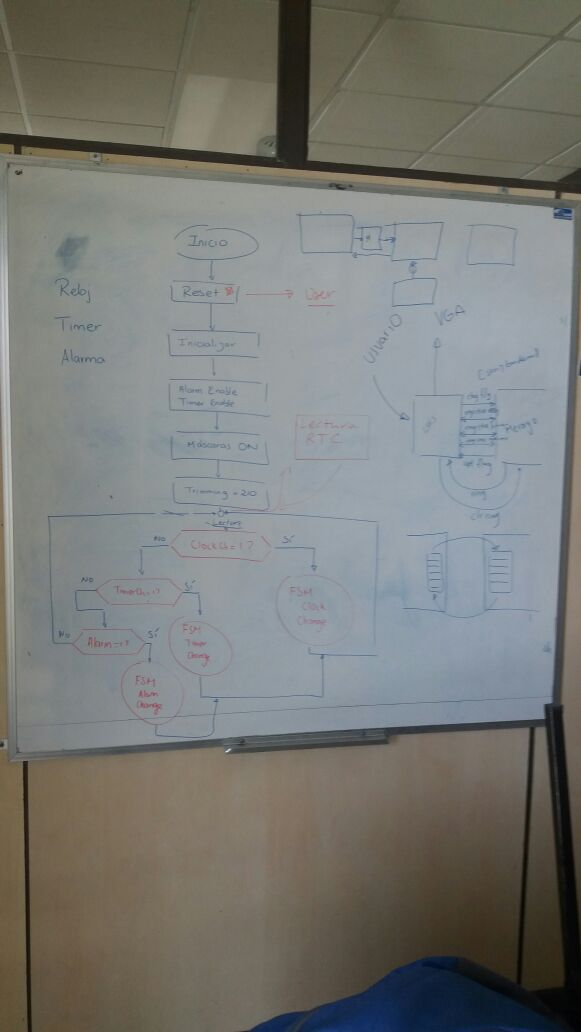
\includegraphics[width=14cm]{Img/rtcdiagramaflujo.jpeg}
	\caption{Diagrama de flujo para el control del RTC}
	\label{fig:RTCdiagramaflujo}
\end{figure}

\newpage

% Nueva entrada
\begin{flushright}
	\begin{large}
		\textbf{Fecha: 2 de Septiembre}\\[5ex]
	\end{large}
\end{flushright}


\noindent \textbf{Integrantes:} Keylor Mena \\[1ex]
\textbf{Hora:} ---\\[1ex]
\textbf{Actividad:} \\[2ex]

ACTUALIZACION REQUERIDA \\[2ex]

\newpage
% Nueva entrada
\begin{flushright}
	\begin{large}
		\textbf{Fecha: 3 de Septiembre}\\[5ex]
	\end{large}
\end{flushright}

\noindent \textbf{Integrantes:} Luis Leon \\[1ex]
\textbf{Hora:} 13:00 - 16:00 \\[1ex]
\textbf{Actividad:} \\[2ex]

Se hizo el diseño del sistema, que incorpora la etapa de control de acceso a la memoria por parte del control de usuario y el RTC. Además, se incorporó el módulo VGA como parte del control de memoria. Esto se puede ver en la figura \ref{fig:sysdesign1} \\

\begin{figure}[hbtp]
	\centering
	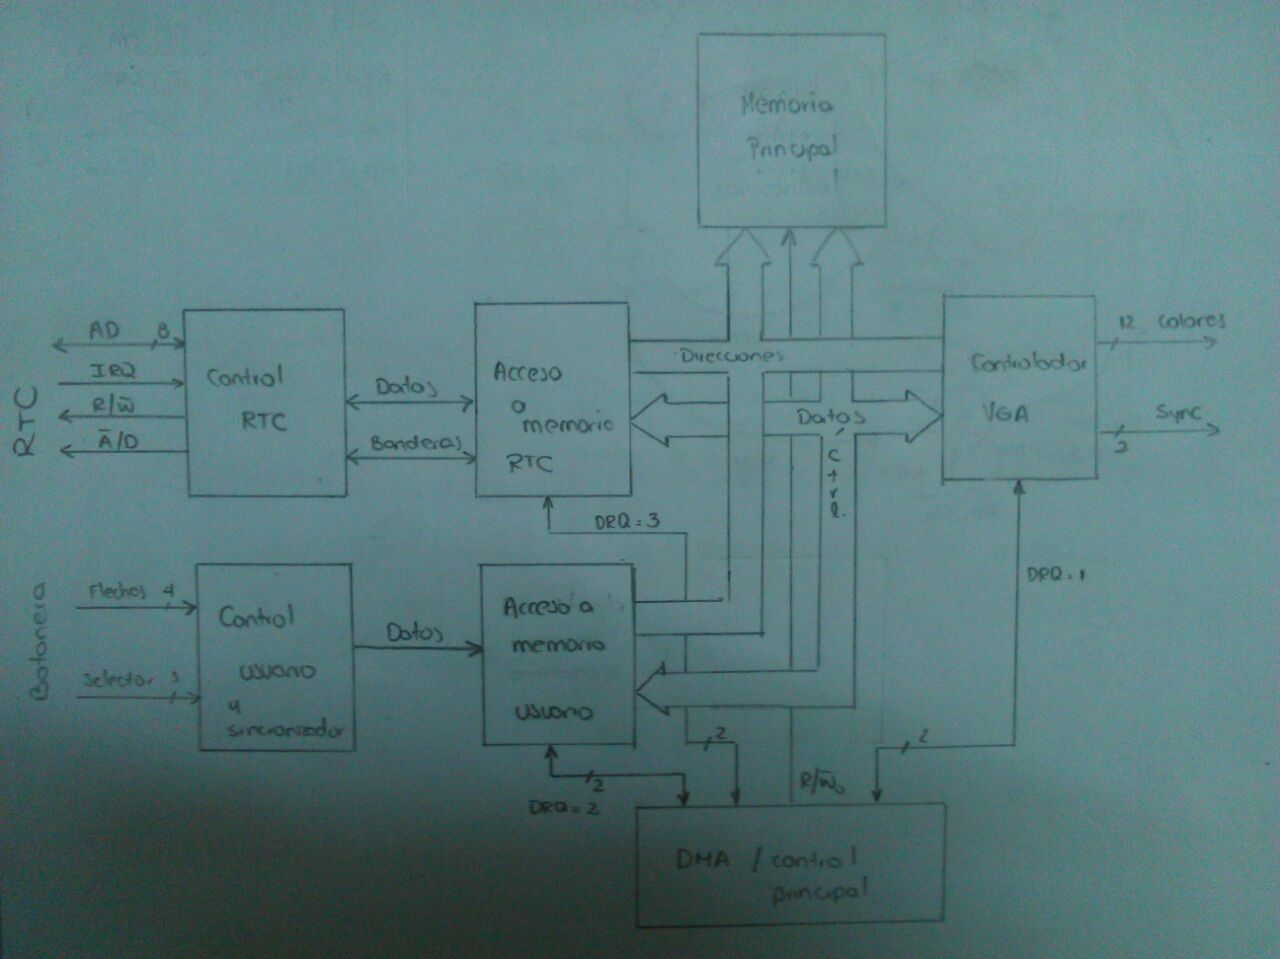
\includegraphics[width=16cm]{Img/sysdesign1.jpeg}
	\caption{Diagrama general del sistema}
	\label{fig:sysdesign1}
\end{figure}

En cuando al acceso a la memoria, esta se regirá por una FSM (máquina de estados), cuyos diseños se presentan el las figuras \ref{fig:mainctrl1} y \ref{fig:mainctrl2}.\\

\begin{figure}[hbtp]
	\centering
	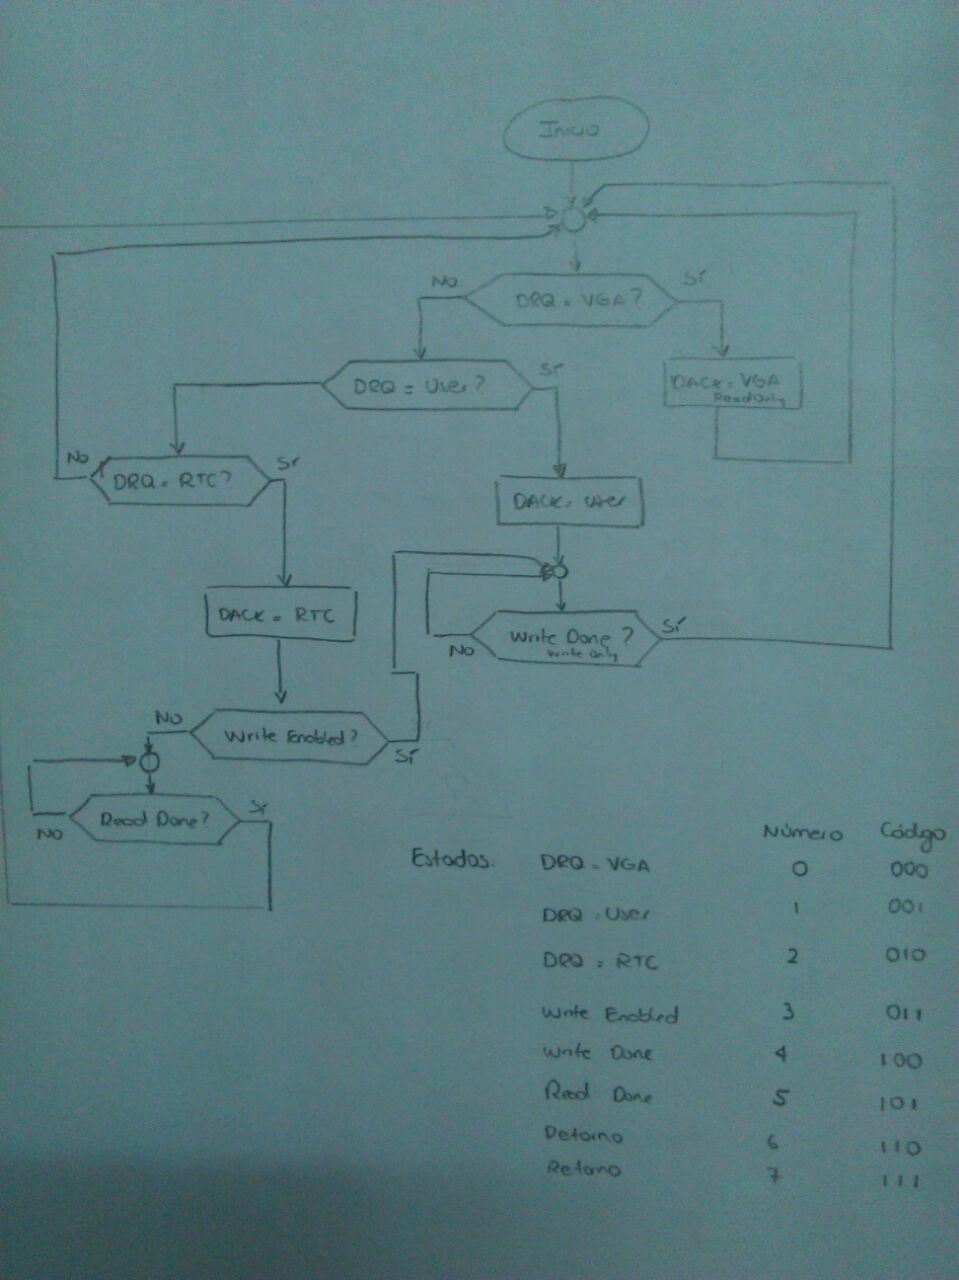
\includegraphics[width=16cm]{Img/mainctrl1.jpg}
	\caption{Diagrama de flujo de la máquina de estados principal}
	\label{fig:mainctrl1}
\end{figure}

\begin{figure}[hbtp]
	\centering
	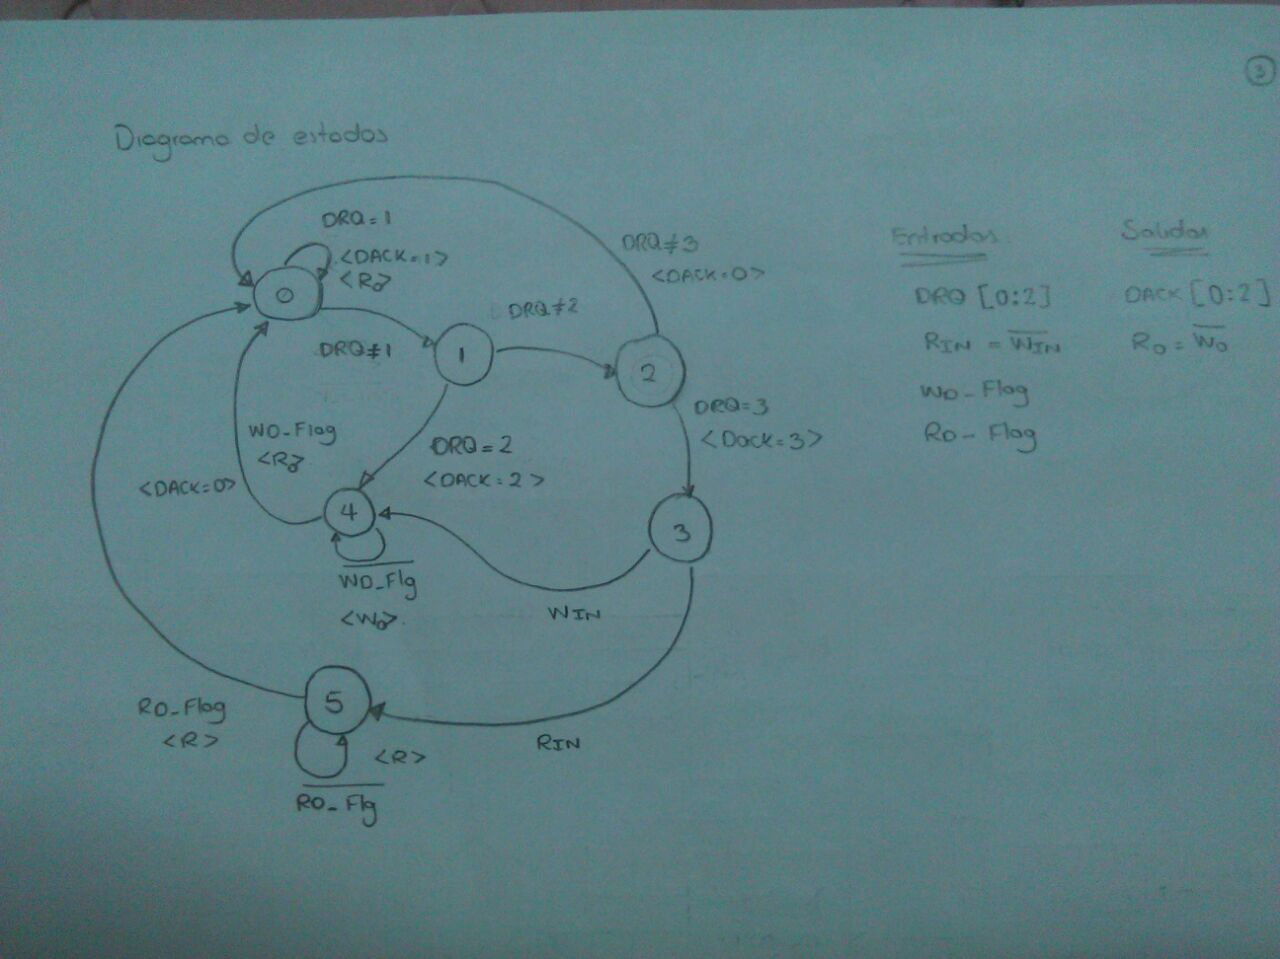
\includegraphics[width=16cm]{Img/mainctrl2.jpg}
	\caption{Diagrama de estados de la máquina de estados principal}
	\label{fig:mainctrl2}
\end{figure}	

\noindent \textbf{Enlaces de interés:} 
http://bit.ly/2c3durR

\newpage
% Nueva entrada
\begin{flushright}
	\begin{large}
		\textbf{Fecha: 4 de Septiembre}\\[5ex]
	\end{large}
\end{flushright}

\noindent \textbf{Integrantes:} keylor Mena \\[1ex]
\textbf{Hora:} 13:00 - 16:00 \\[1ex]
\textbf{Actividad:} \\[2ex]

Se programo el nuevo registro dual con actualizacion controlada, este permite aislar etapas principales teniendo registros individuales entre ellas y actualizando estos con señales o banderas


\newpage
% Nueva entrada
\begin{flushright}
	\begin{large}
		\textbf{Fecha: 5 de Septiembre}\\[5ex]
	\end{large}
\end{flushright}

\noindent \textbf{Integrantes:} Luis Leon \\[1ex]
\textbf{Hora:} 14:30 - 17:00 \\[1ex]
\textbf{Actividad:} \\[2ex]

Se hicieron los diagramas de bloques del control VGA y del control de usuario. Estos diagramas contienen unidades de control y otras subunidades que deben ser descritas, por ello, se hace un pequeño índice de los elaborado el día de hoy. \\

\begin{itemize}
	\item Control VGA: 
		\subitem Diagrama de bloques (Figura \ref{fig:BloquesVGA1}) 
		\subitem Diagrama de flujo (Figura \ref{fig:FlujoVGA1})
		\subitem Diagrama de bloques direccionamiento (Figura \ref{fig:DireccionamientoBloquesVGA1})
		\subitem Diagrama de flujo direccionamiento (Figura \ref{fig:DireccionamientoFlujoVGA1})
	\item Control de Usuario:
		\subitem Diagrama de bloques (Figura \ref{fig:BloquesUsuario1})
		\subitem Diagrama de flujo (Figura \ref{fig:FlujoUsuario1})
\end{itemize}

Finalmente, por algunos problemas de salud, se ha decidido colaborar en la parte de implementación del código en Verilog y al diseño del control VGA. Se expondrá a los compañeros la situación y, por otro lado, se aclararán algunos aspectos de memoria que deben ser discutidos para que haya armonía en la implementación.

\begin{figure}[hbtp]
	\centering
	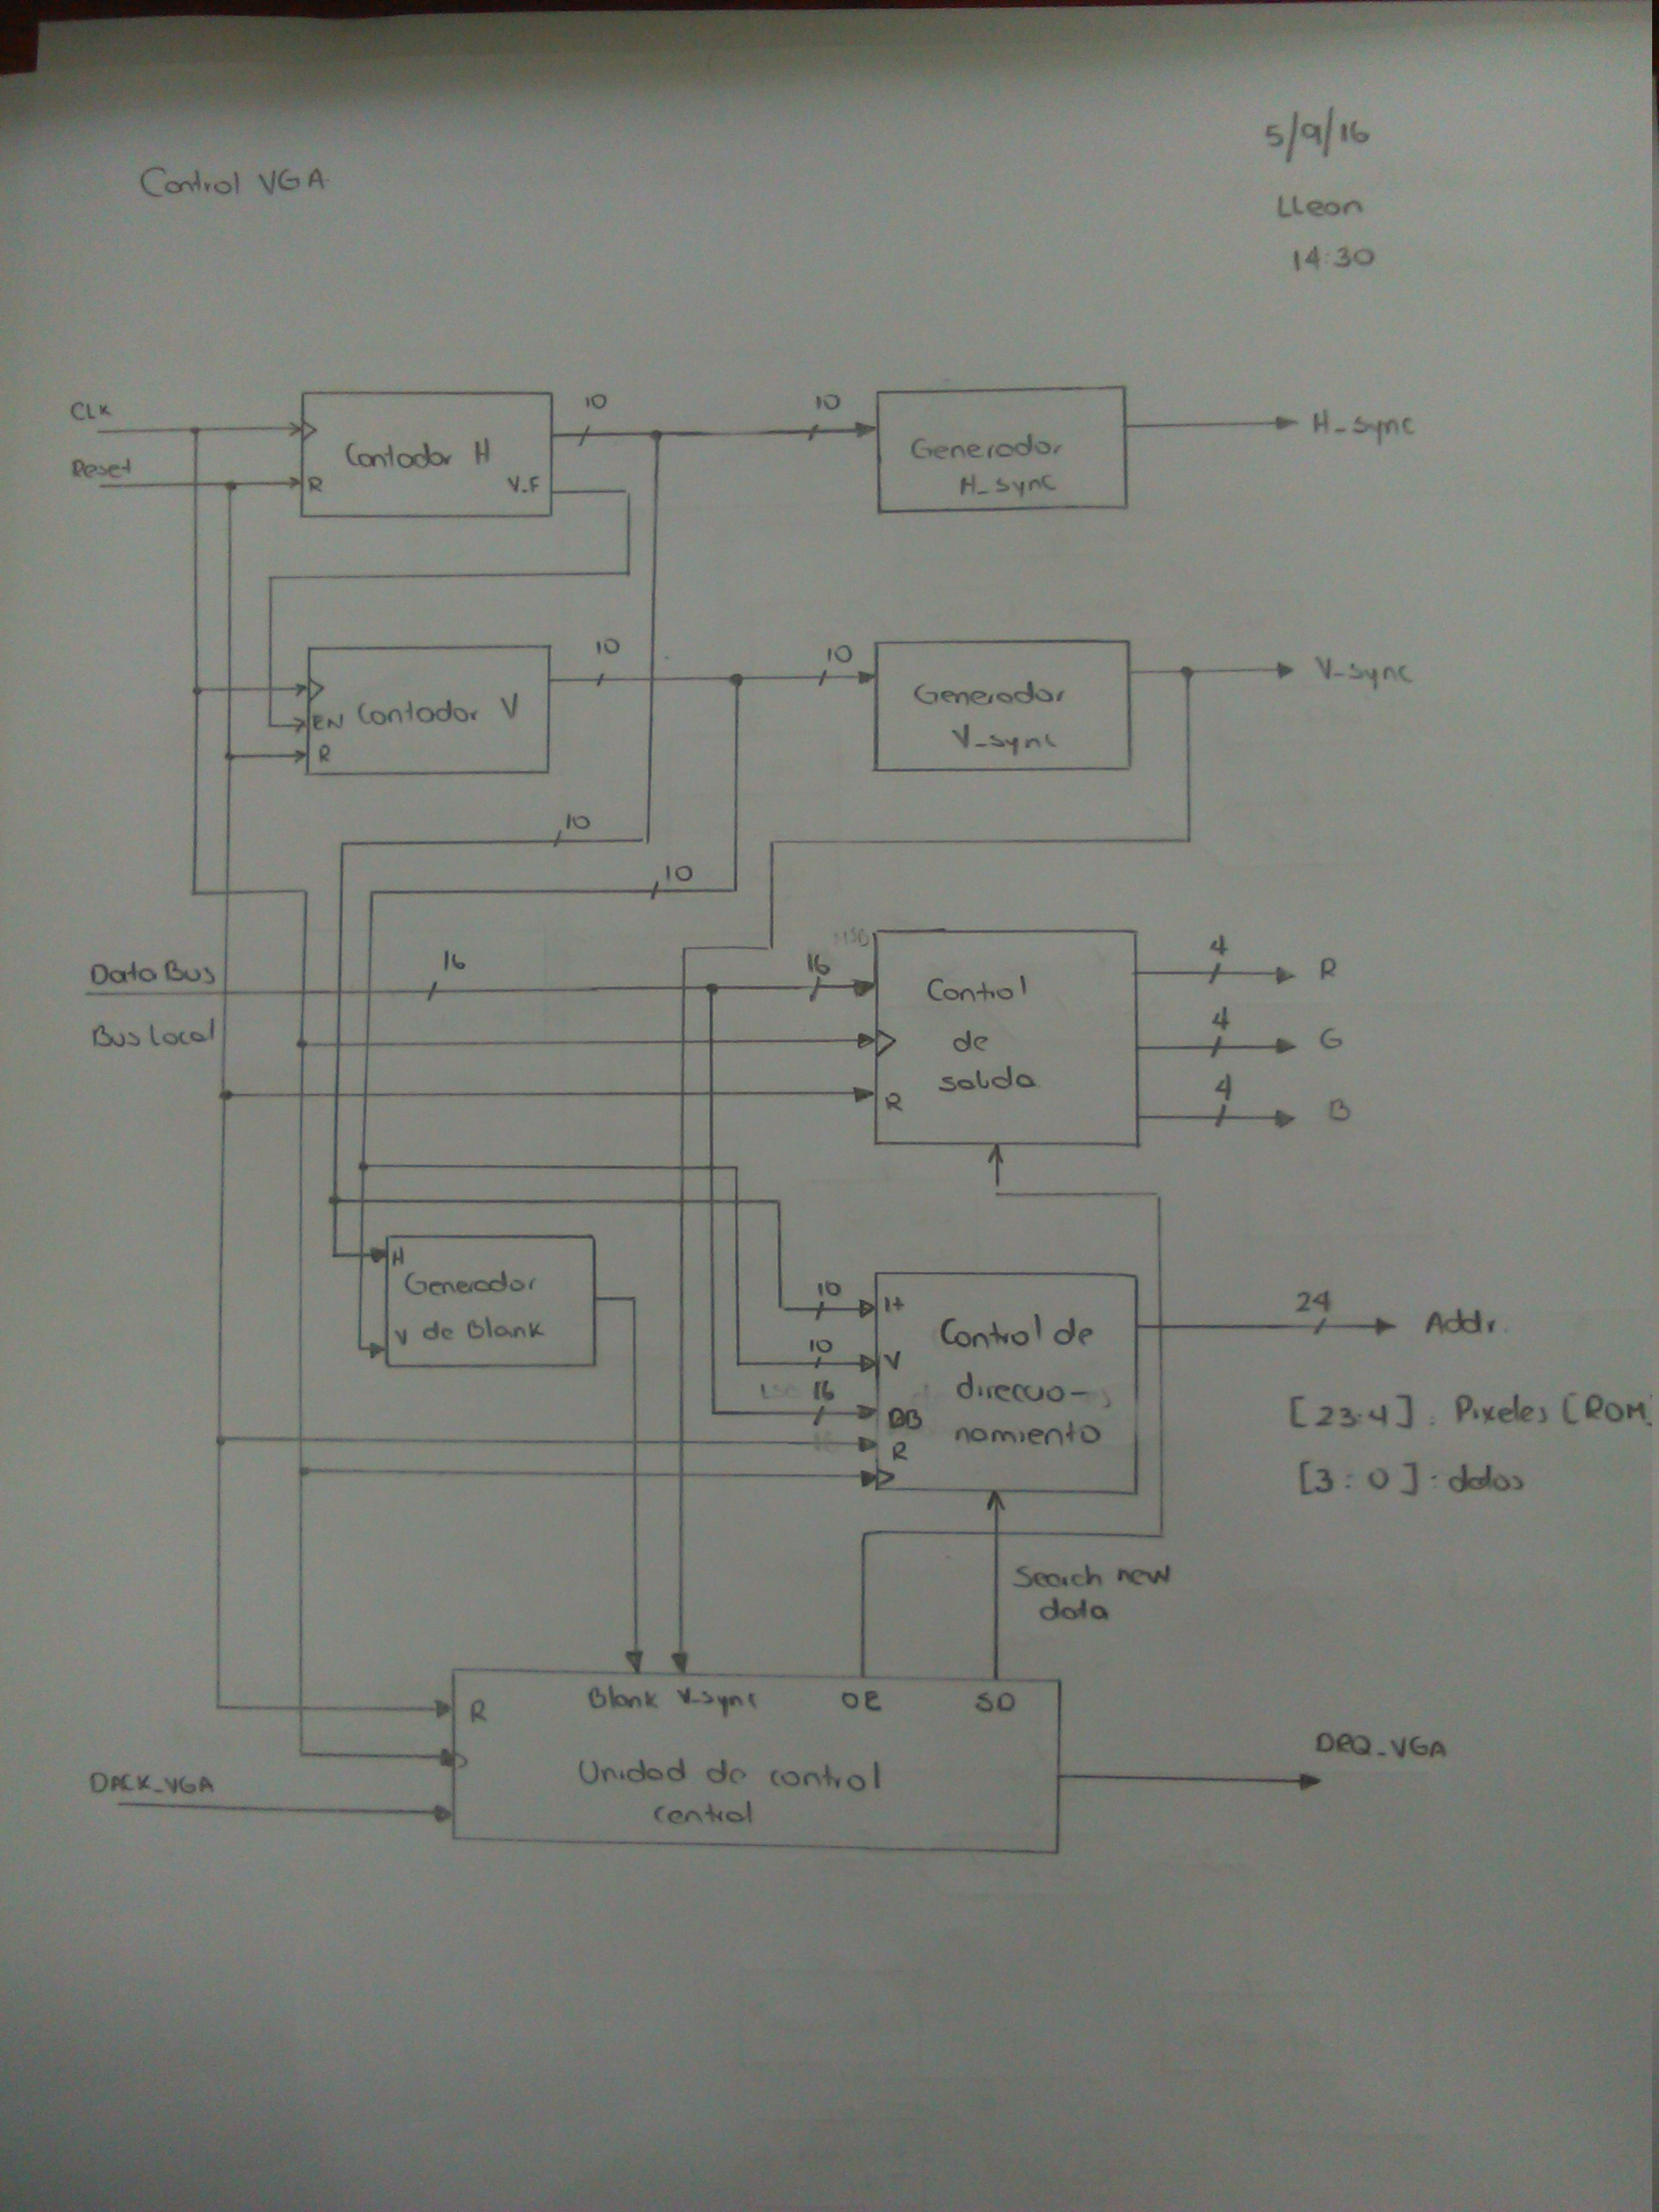
\includegraphics[width=16cm,height=20cm]{Img/ControlVGABloques.jpg}
	\caption{Diagrama de bloques del Control VGA}
	\label{fig:BloquesVGA1}
\end{figure}

\begin{figure}[hbtp]
	\centering
	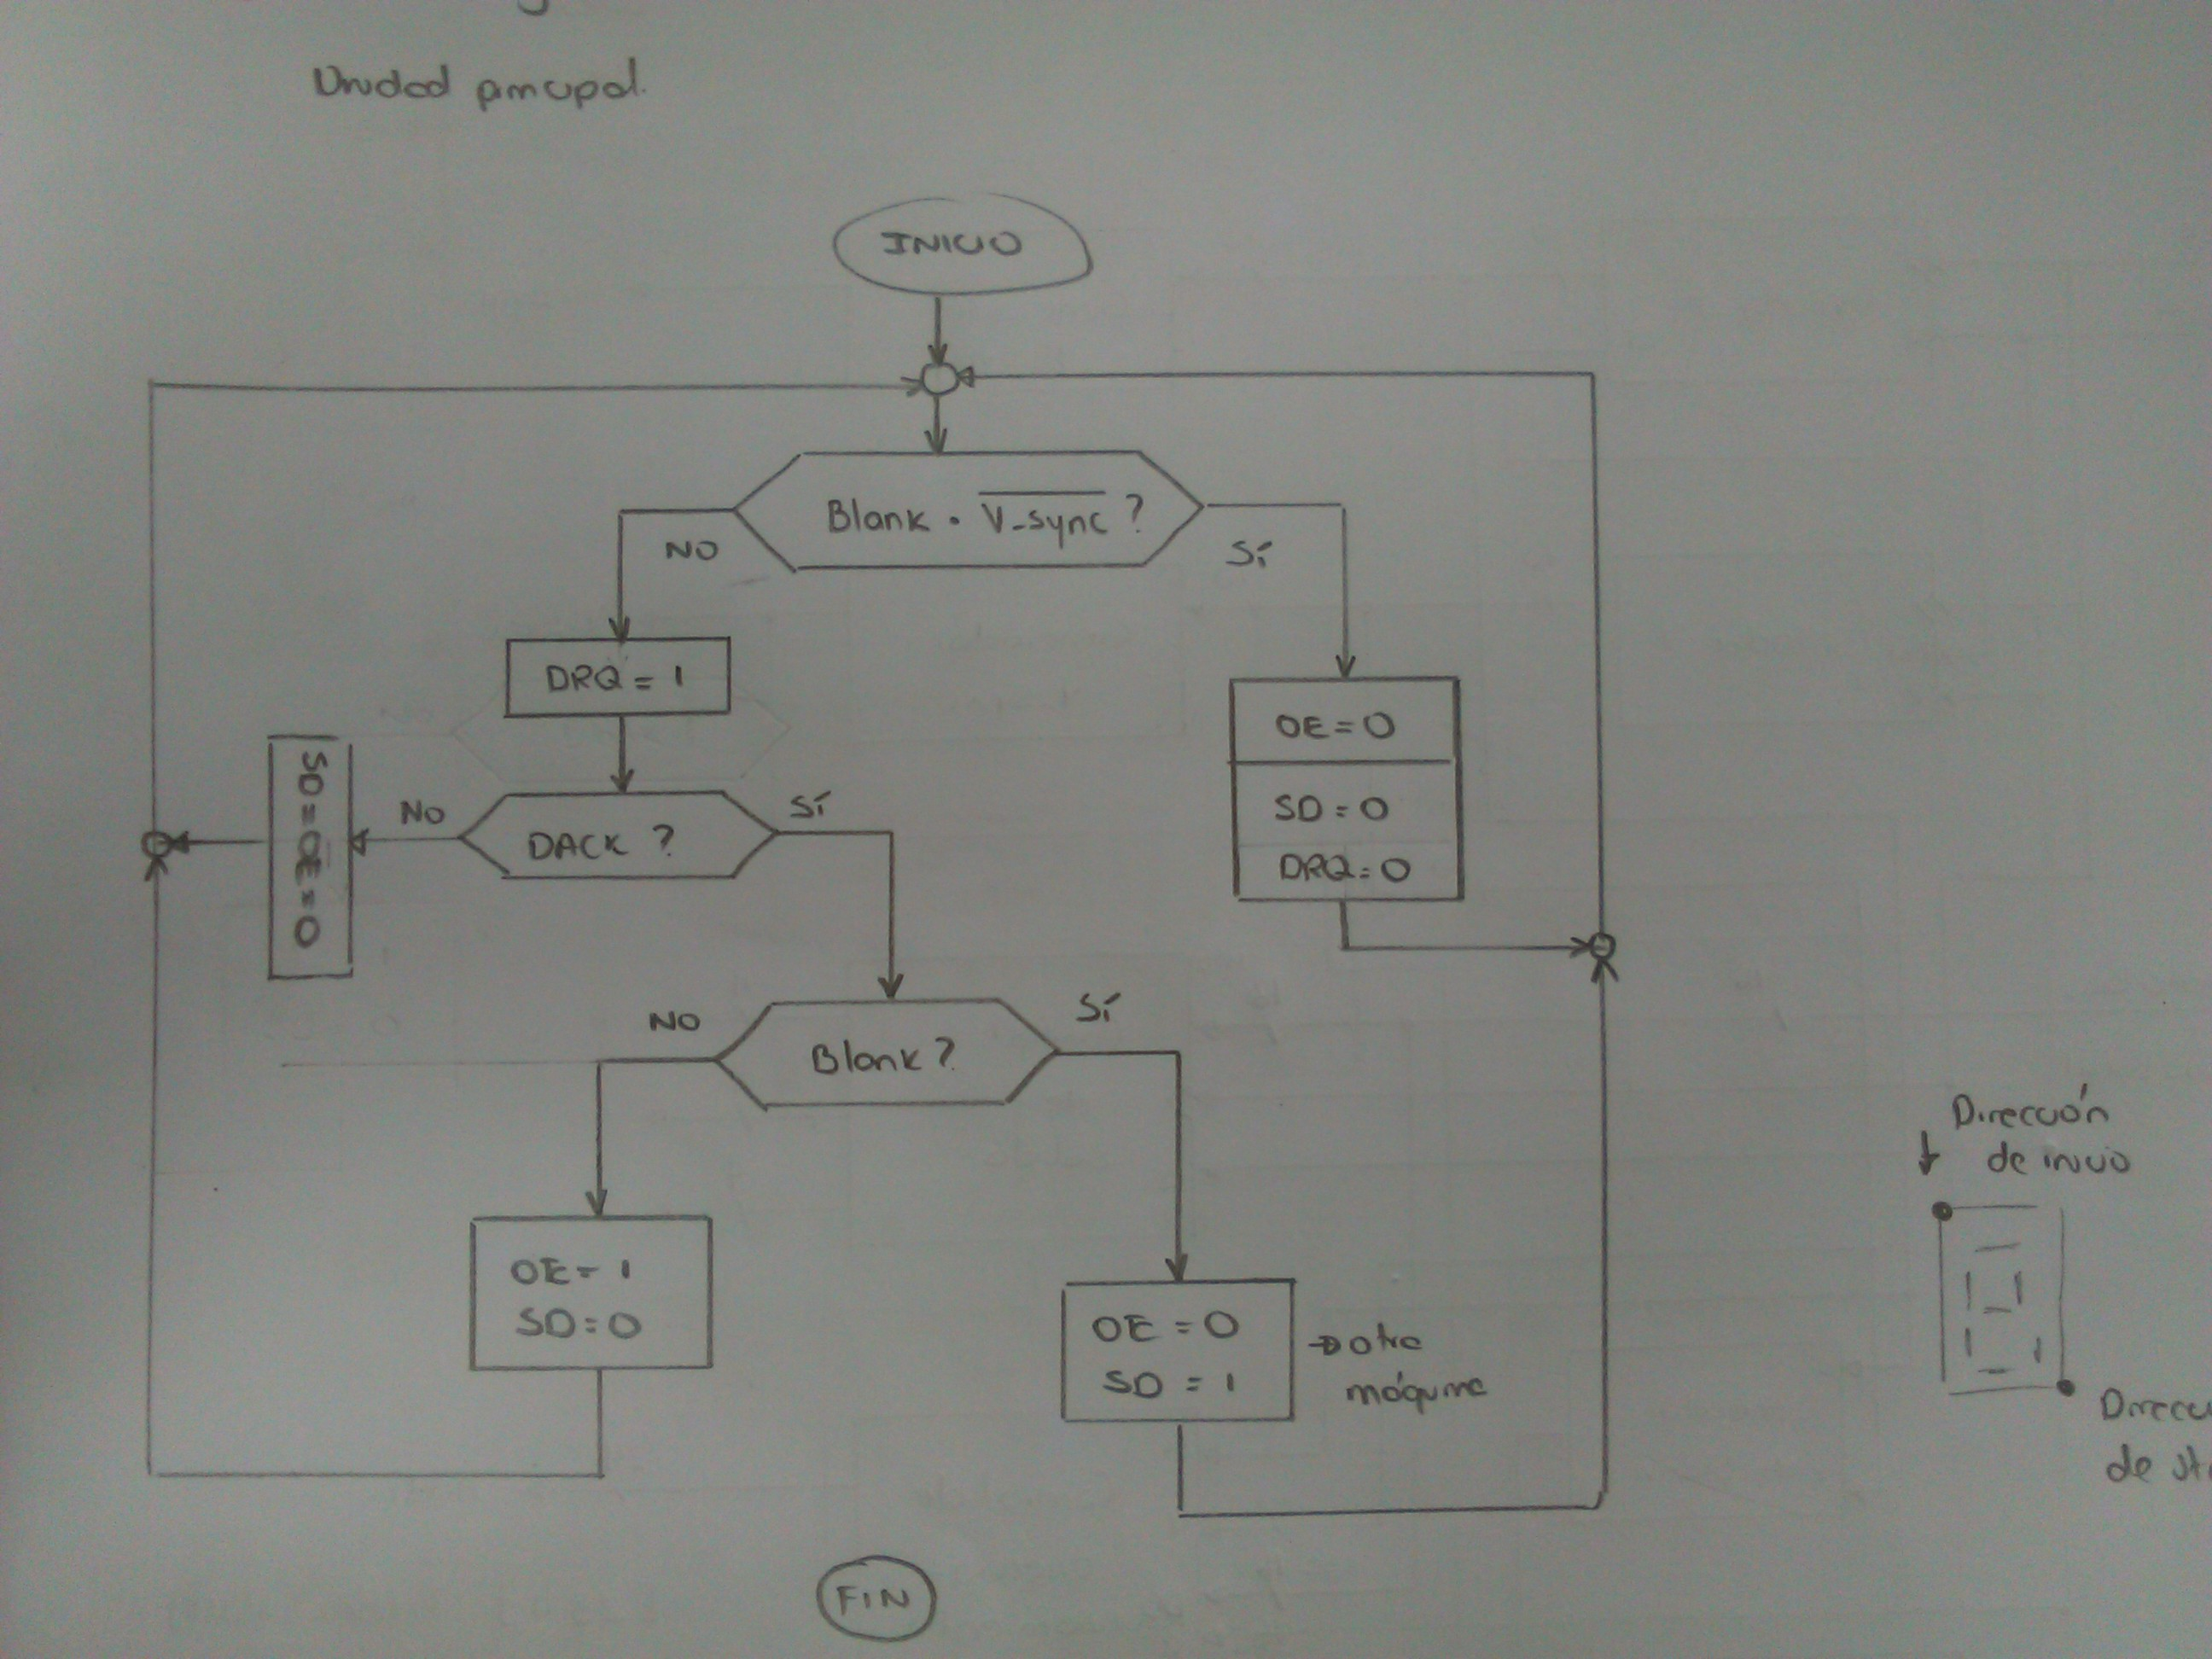
\includegraphics[width=15cm,height=10cm]{Img/ControlVGAFlujo.jpg}
	\caption{Diagrama de Flujo del Control VGA}
	\label{fig:FlujoVGA1}
\end{figure}

\begin{figure}[hbtp]
	\centering
	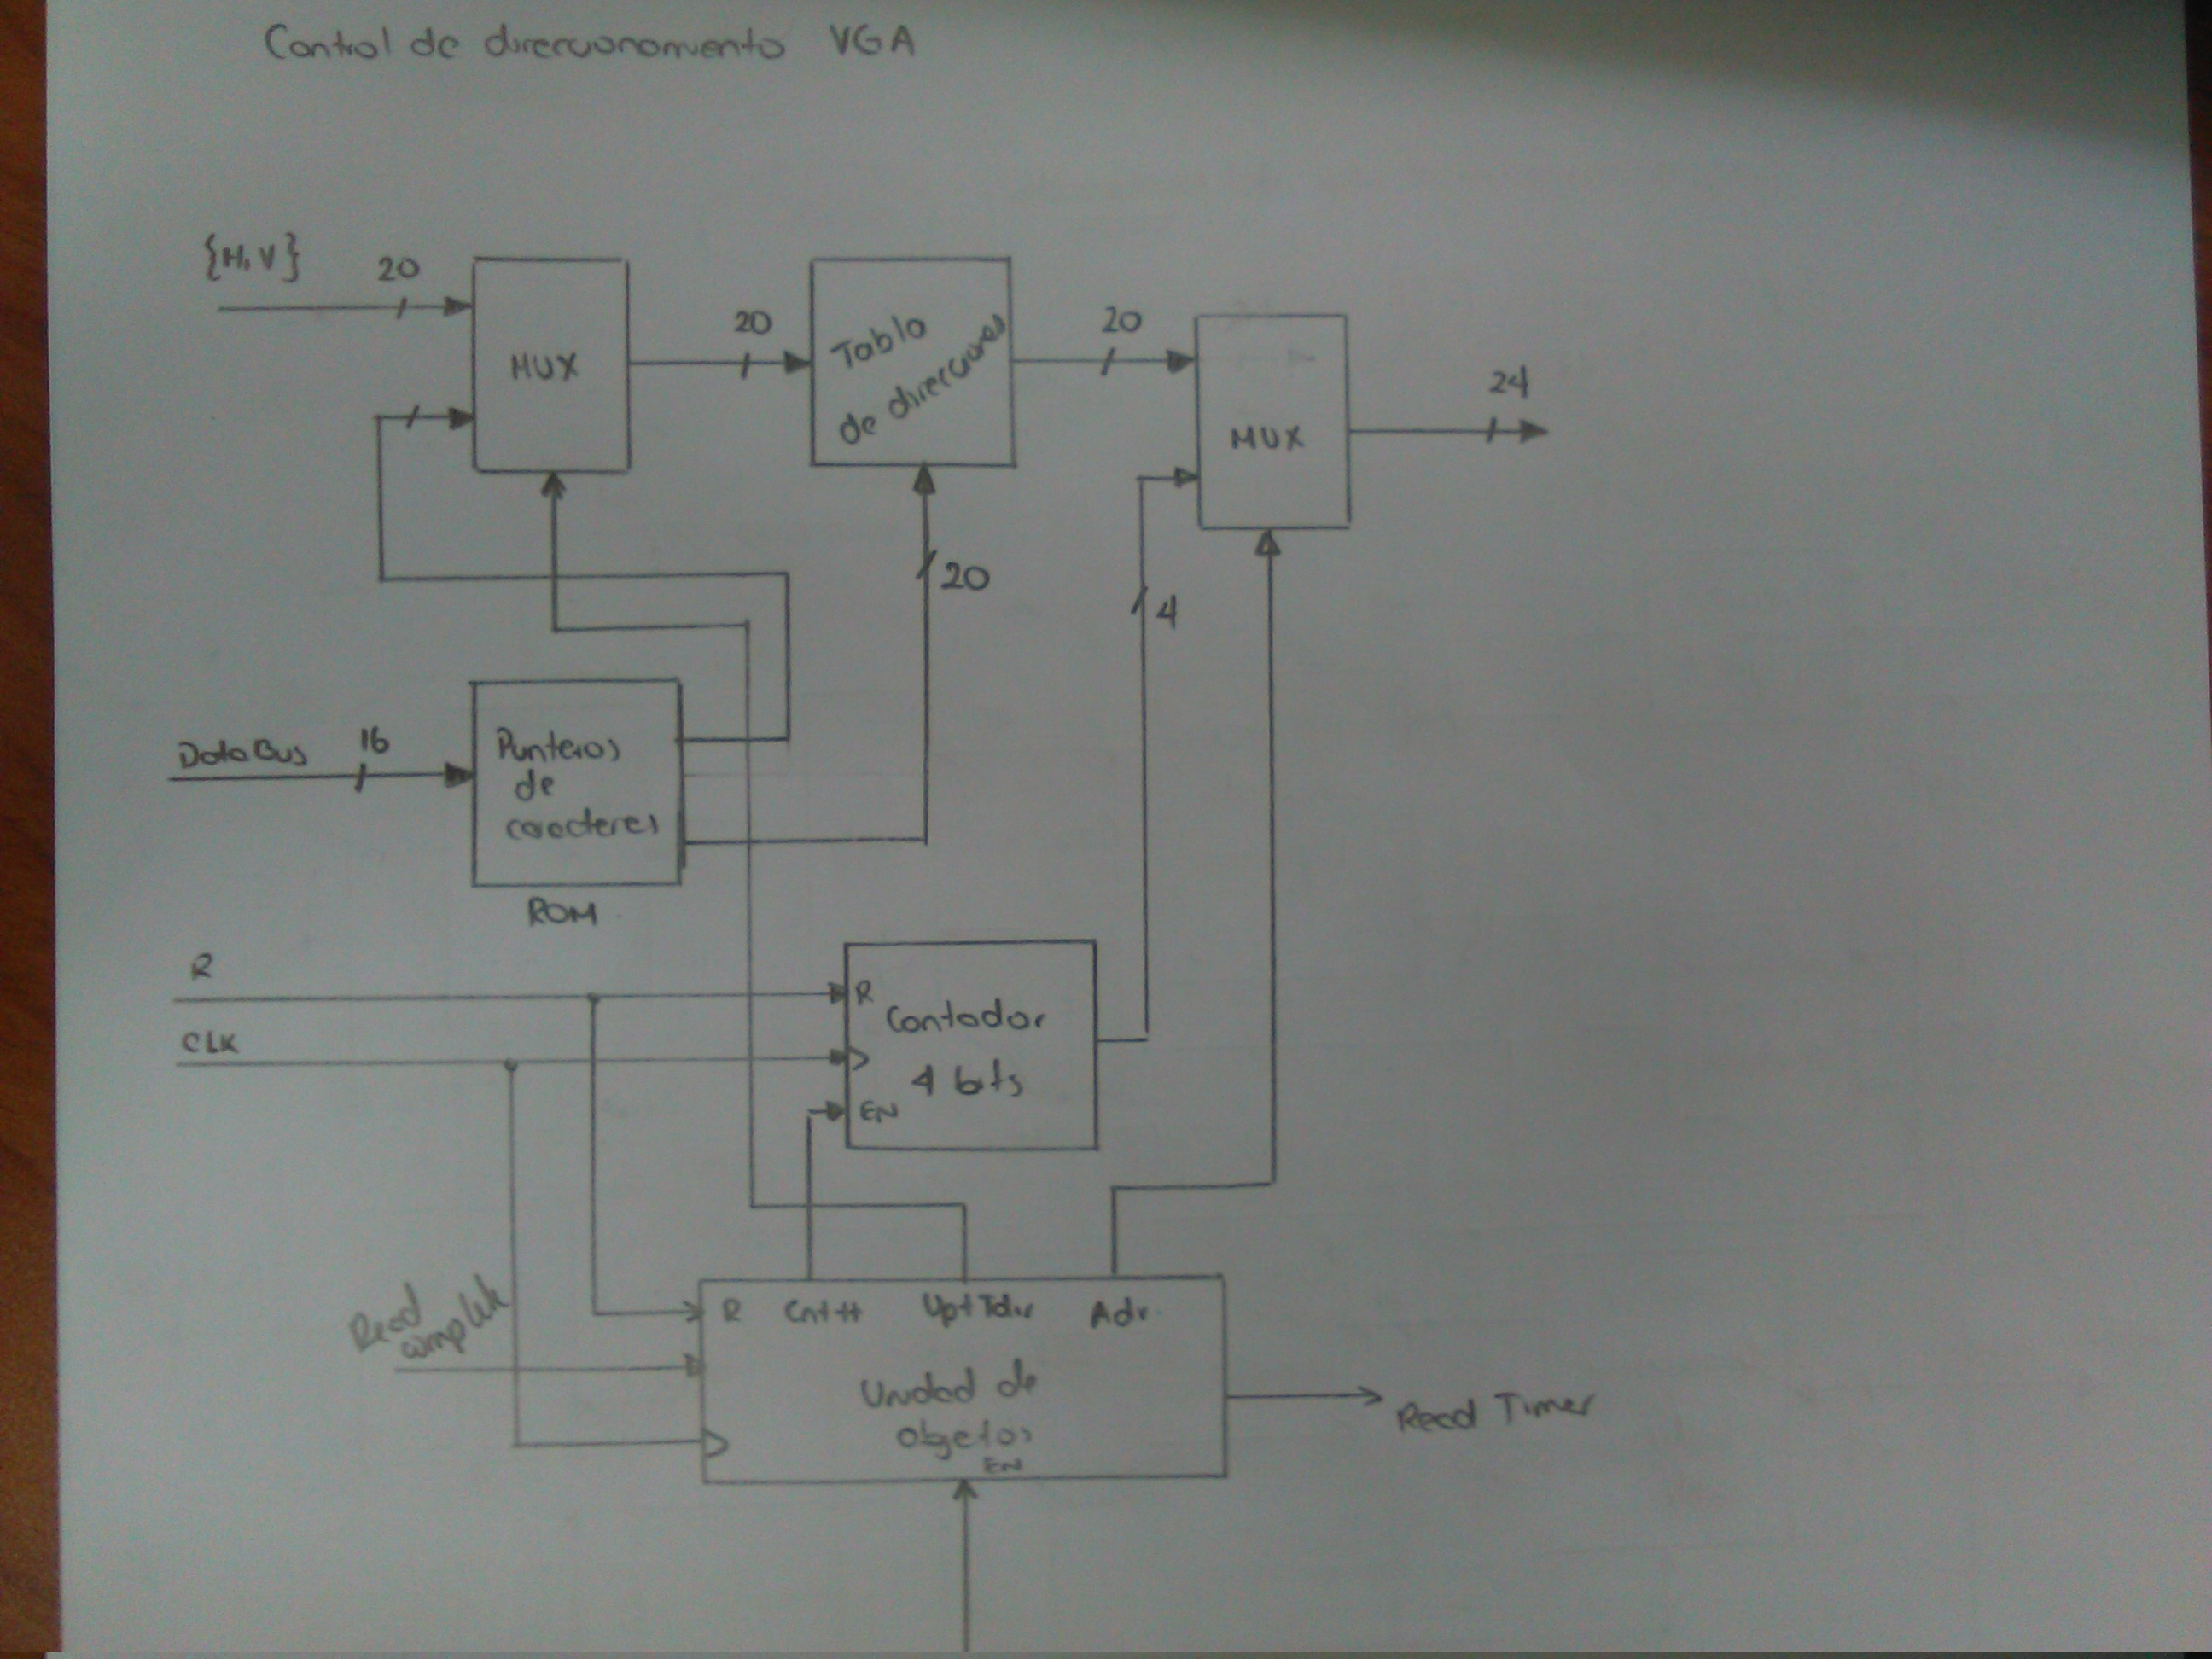
\includegraphics[width=15cm]{Img/ControlDireccionamientoVGABloques.jpg}
	\caption{Diagrama de Bloques del Control VGA - Sección de Direccionamiento}
	\label{fig:DireccionamientoBloquesVGA1}
\end{figure}

\begin{figure}[hbtp]
	\centering
	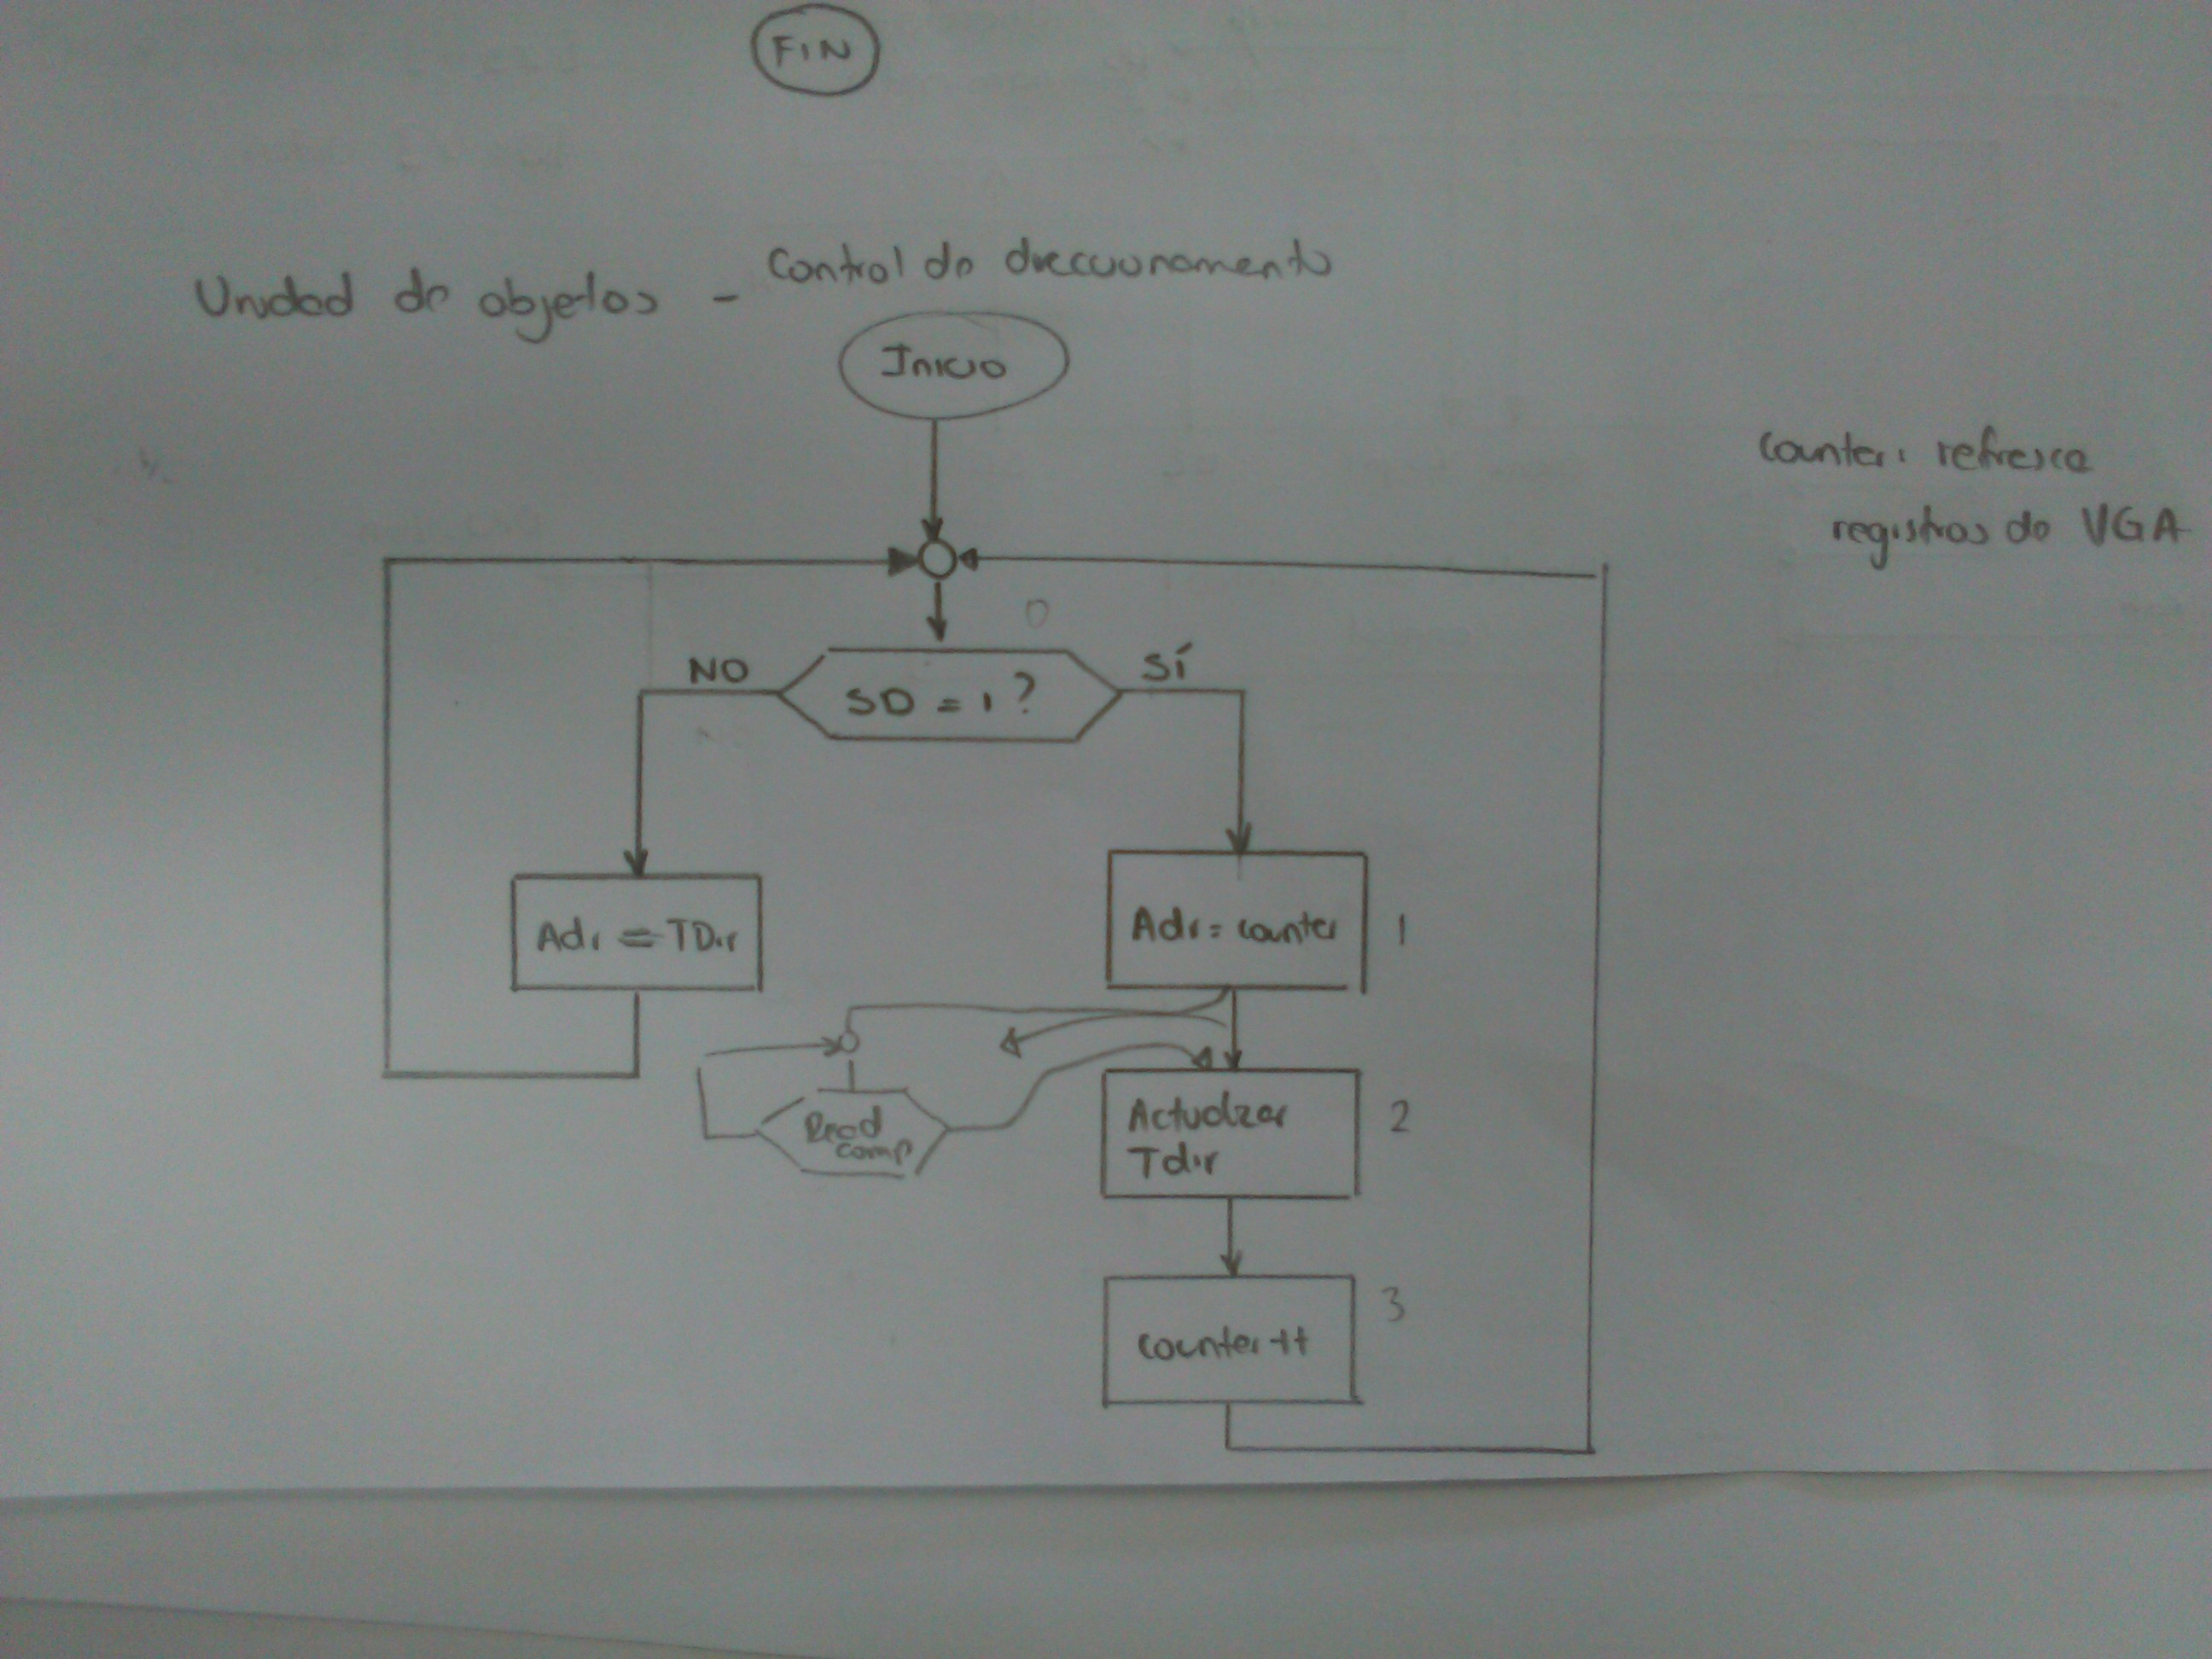
\includegraphics[width=15cm]{Img/ControlDireccionamientoVGAFlujo.jpg}
	\caption{Diagrama de Bloques del Control VGA - Sección de Direccionamiento}
	\label{fig:DireccionamientoFlujoVGA1}
\end{figure}

\begin{figure}[hbtp]
	\centering
	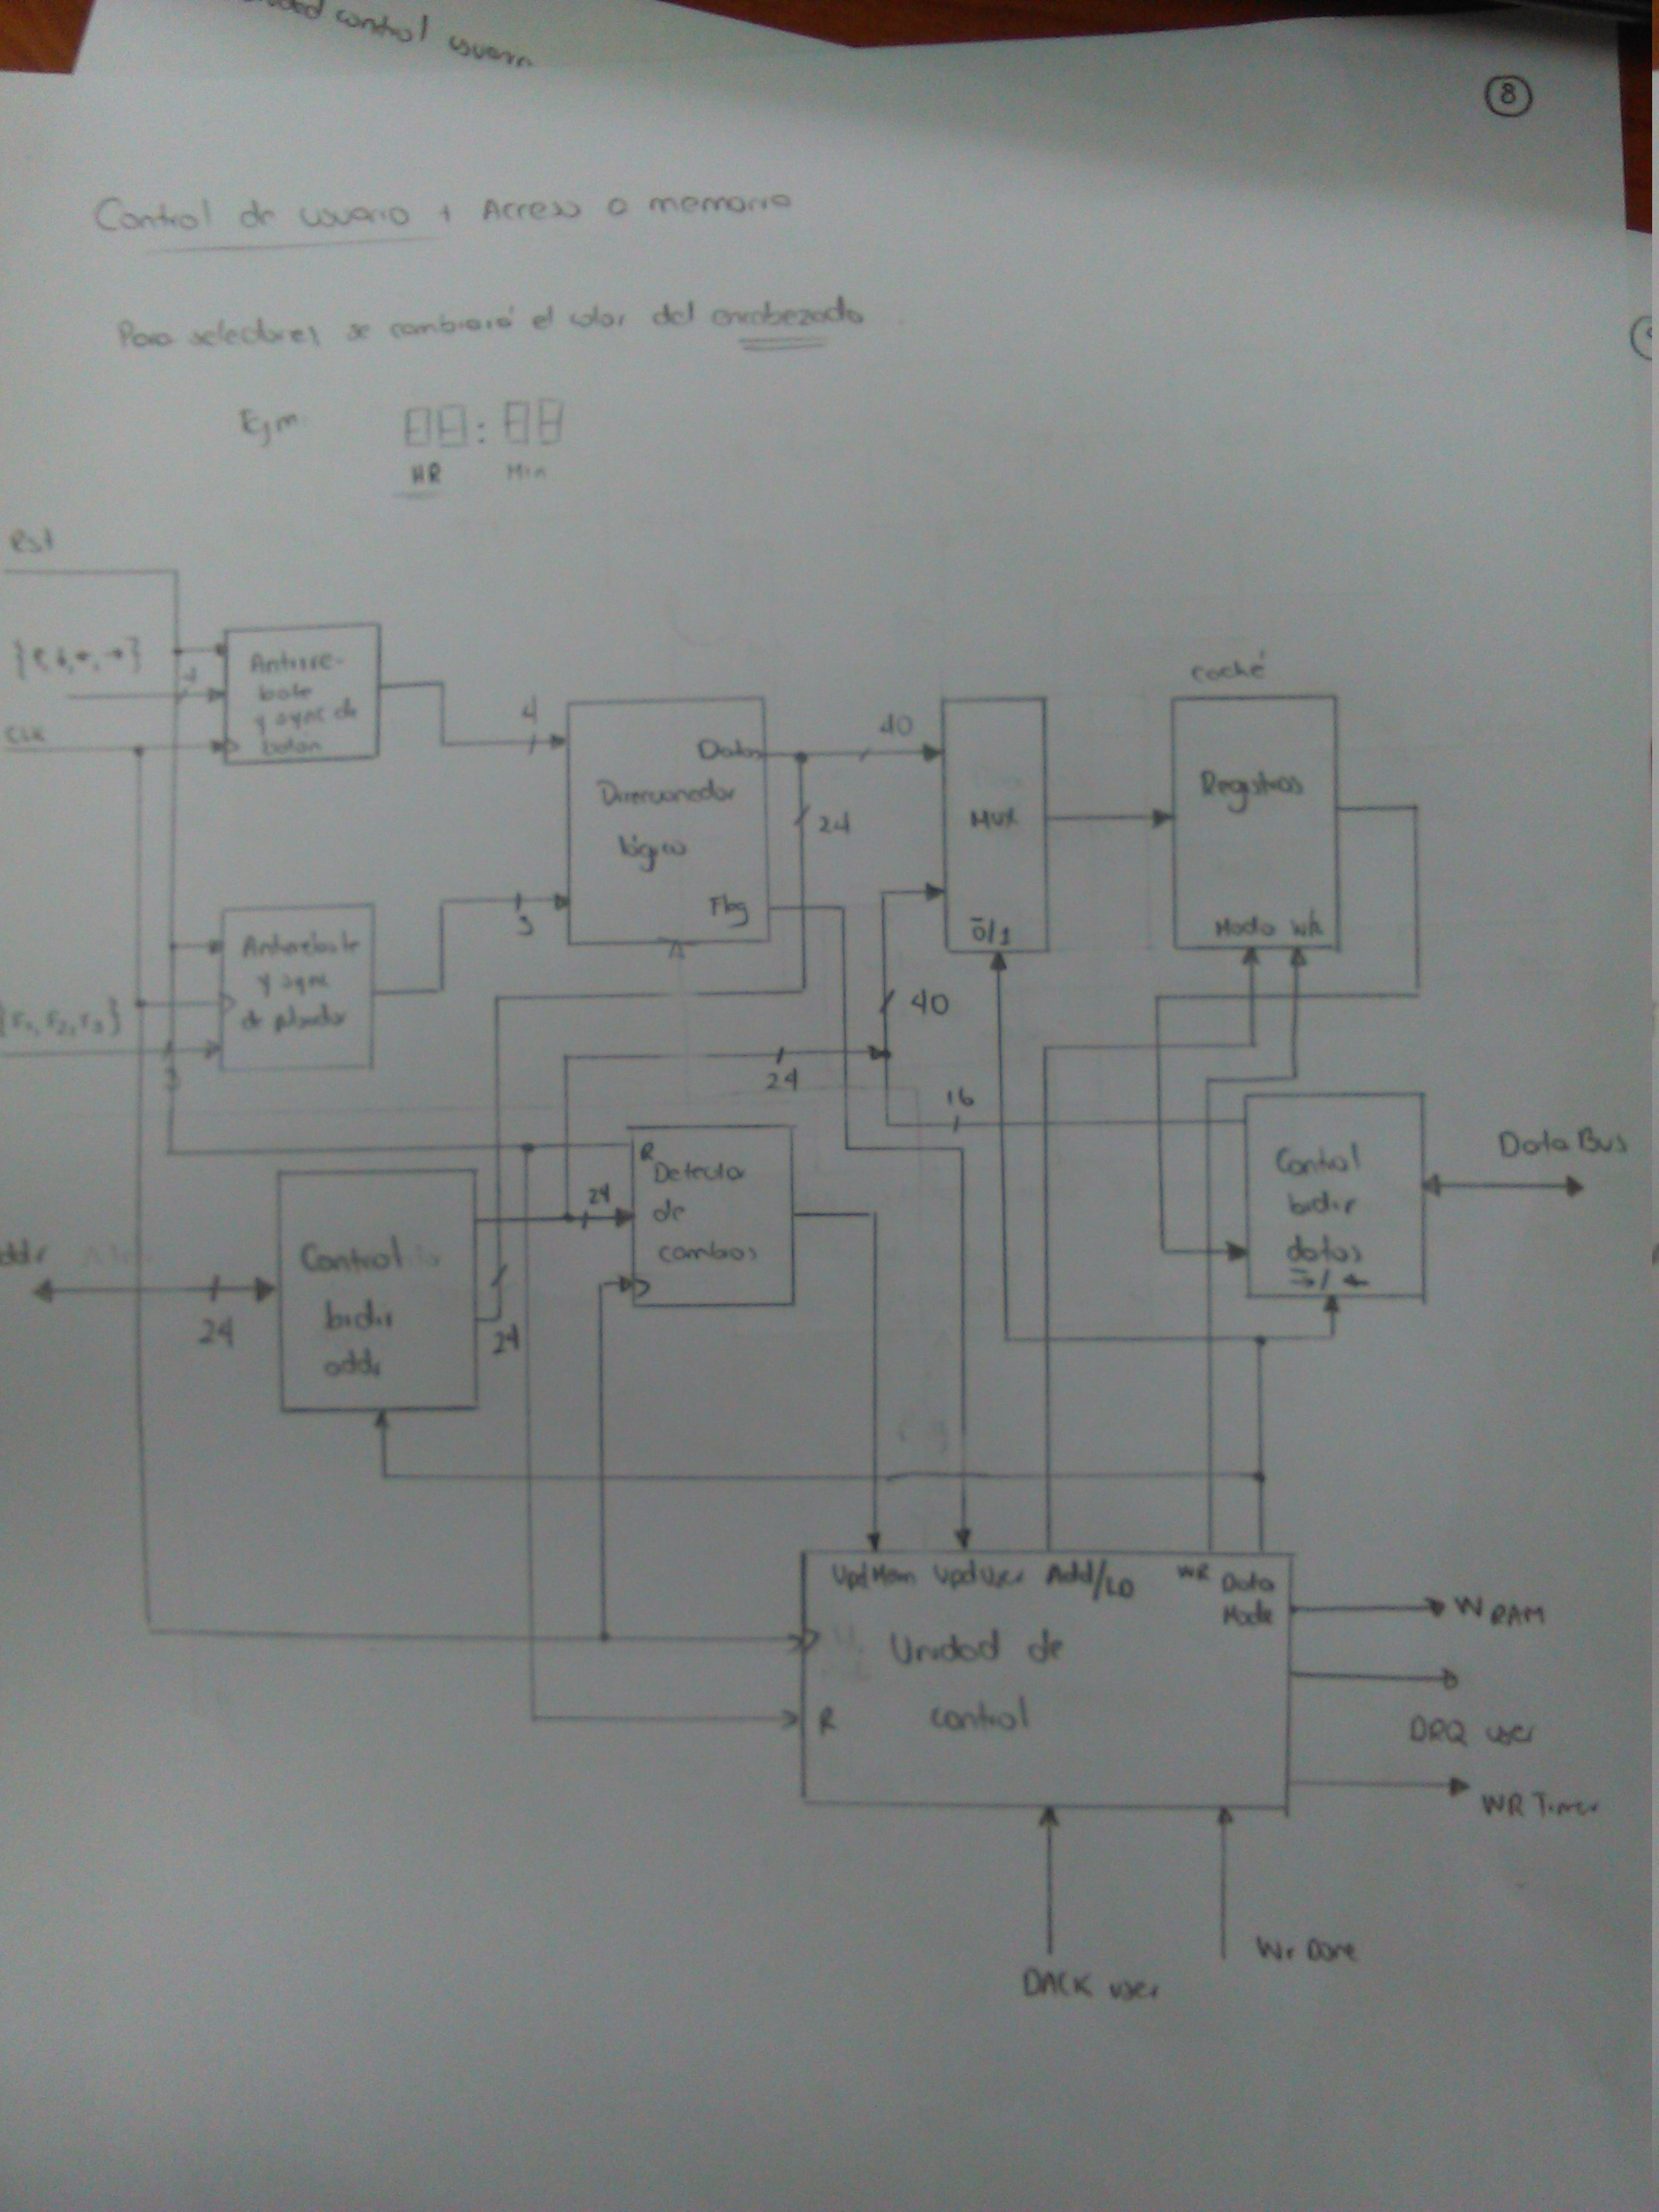
\includegraphics[width=15cm]{Img/ControlUsuarioBloques.jpg}
	\caption{Diagrama de Bloques del Control de Usuario}
	\label{fig:BloquesUsuario1}
\end{figure}

\begin{figure}[hbtp]
	\centering
	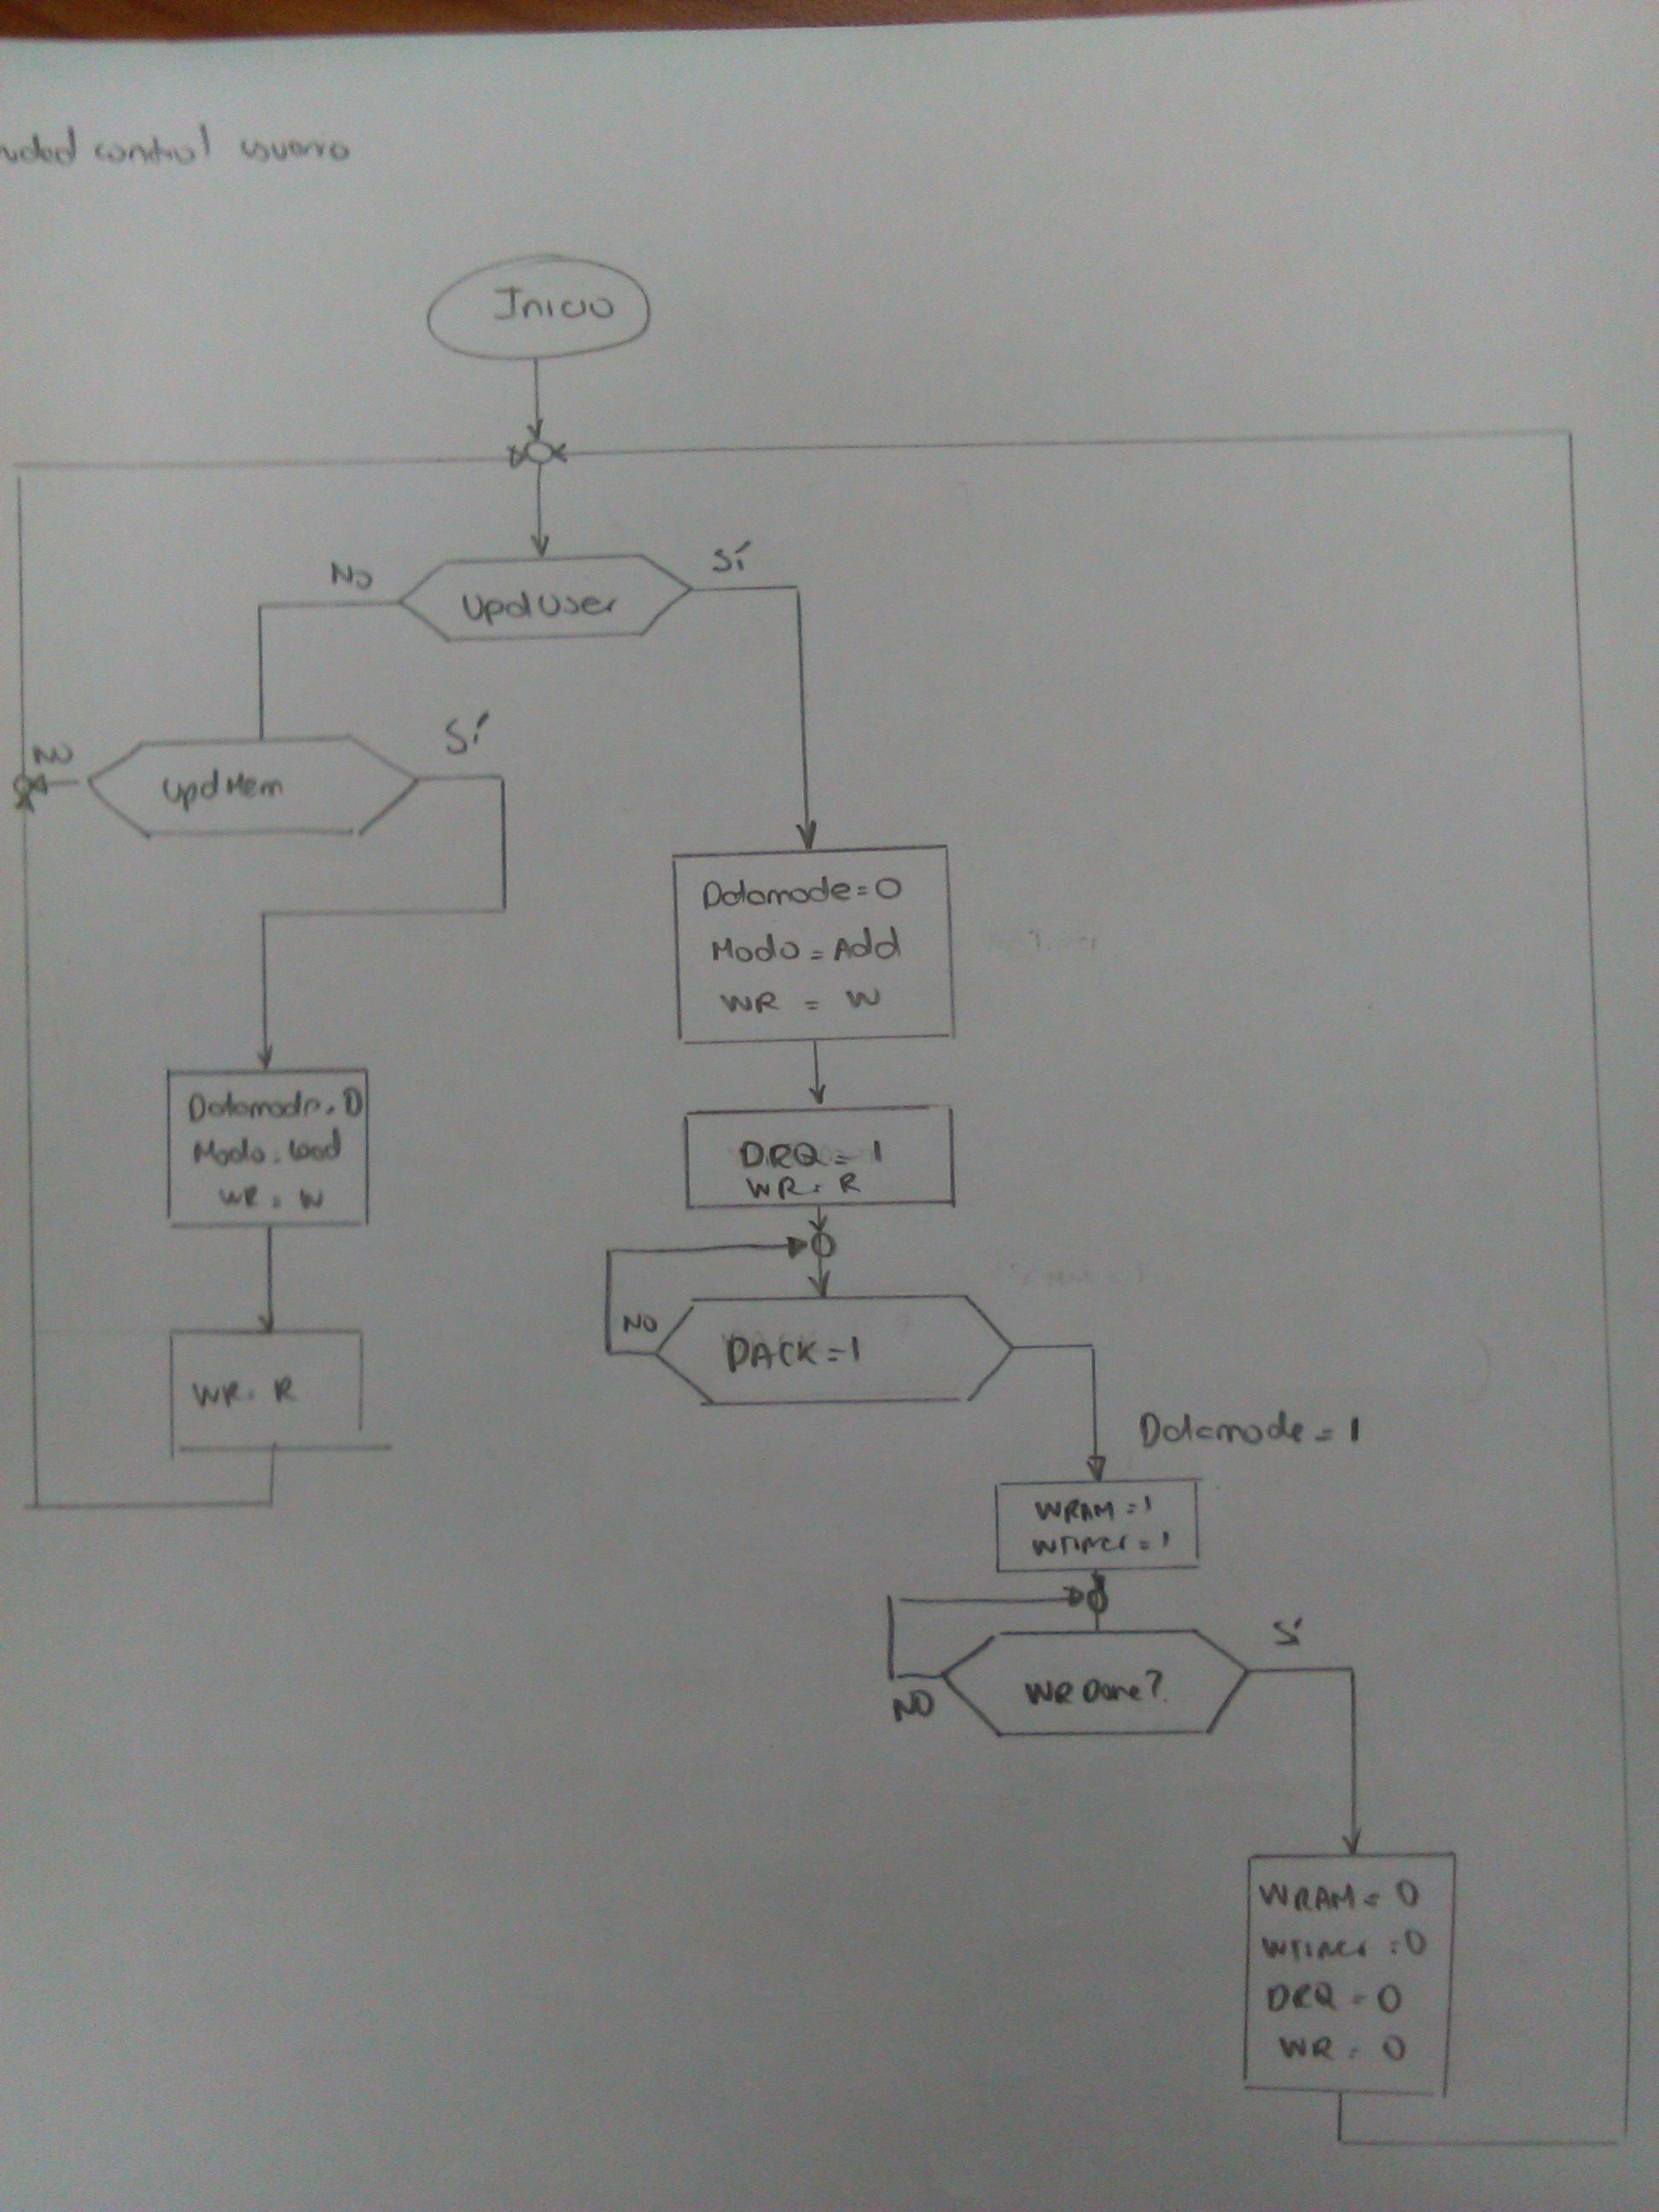
\includegraphics[width=15cm]{Img/ControlUsuarioFlujo.jpg}
	\caption{Diagrama de Flujo del Control de Usuario}
	\label{fig:FlujoUsuario1}
\end{figure}

\begin{flushright}
	\begin{large}
		\textbf{Fecha: 3 de Septiembre}\\[5ex]
	\end{large}
\end{flushright}

\noindent \textbf{Integrantes:} Luis Merayo \\[1ex]
\textbf{Hora:} 21:00 - 22:00 \\[1ex]
\textbf{Actividad:} \\[2ex]

Actividad: Se realizó un primer diseño del control del RTC, por lo que se resaltó la ruta de datos e inicialmente se crearon tres máquinas de estado, una de escritura, otra de lectura, y la principal, la cual controla los procedimientos iniciales luego de un reset. También para controlar los tiempos se colocó un contador. Esto se puede ver en la figura \ref{fig:ControlRTC1} \\

\begin{figure}[hbtp]
	\centering
	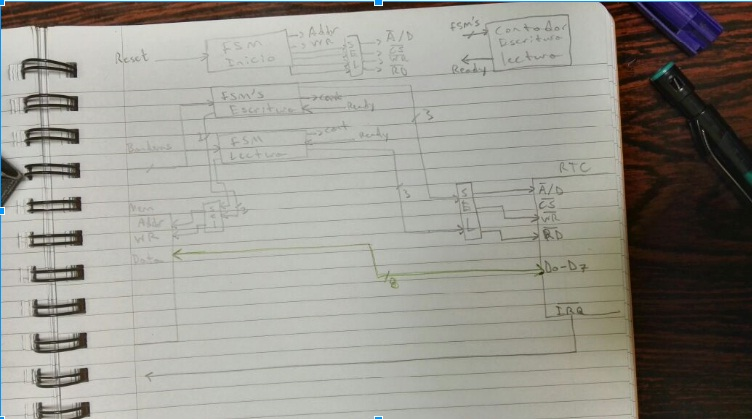
\includegraphics[width=16cm]{Img/ControlRTC1.jpg}
	\caption{Diagrama del control RTC}
	\label{fig:ControlRTC1}
\end{figure}
\end{document}
